% Figure: DeltaSort worst-case movement diagram
\begin{figure}
\centering
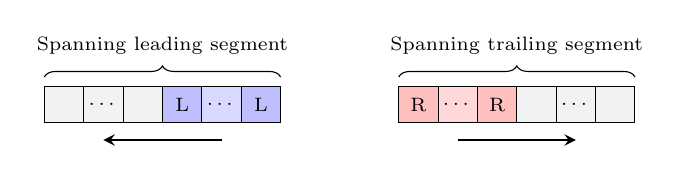
\begin{tikzpicture}[
    cell/.style={minimum width=0.5cm, minimum height=0.45cm, draw, font=\scriptsize, inner sep=0pt, outer sep=0pt, anchor=west},
    dotcell/.style={minimum width=0.5cm, minimum height=0.45cm, draw, font=\scriptsize, inner sep=0pt, outer sep=0pt, anchor=west},
    right/.style={cell, fill=red!25},
    left/.style={cell, fill=blue!25},
    clean/.style={cell, fill=gray!10, font=\scriptsize},
    segbrace/.style={decorate, decoration={brace, amplitude=4pt}},
    seglabel/.style={font=\scriptsize},
]

\def\yarr{0}
\def\cellw{0.5}
\def\xoffset{4.5}

% === LEFT ARRAY: Leading segment (L cluster at right end) ===
\node[clean] at (0, \yarr) {};
\node[dotcell, fill=gray!10] at (\cellw, \yarr) {\dots};
\node[clean] at (2*\cellw, \yarr) {};
\node[left] at (3*\cellw, \yarr) {L};
\node[dotcell, fill=blue!15] at (4*\cellw, \yarr) {\dots};
\node[left] at (5*\cellw, \yarr) {L};

% Brace for left array
\draw[segbrace] (0, 0.35) -- (6*\cellw, 0.35);
\node[seglabel] at (3*\cellw, 0.75) {Spanning leading segment};

% Left arrow below left array
\draw[->, thick, >=stealth] (4.5*\cellw, -0.45) -- (1.5*\cellw, -0.45);


% === RIGHT ARRAY: Trailing segment (R cluster at left end) ===
\node[right] at (\xoffset, \yarr) {R};
\node[dotcell, fill=red!15] at (\xoffset+\cellw, \yarr) {\dots};
\node[right] at (\xoffset+2*\cellw, \yarr) {R};
\node[clean] at (\xoffset+3*\cellw, \yarr) {};
\node[dotcell, fill=gray!10] at (\xoffset+4*\cellw, \yarr) {\dots};
\node[clean] at (\xoffset+5*\cellw, \yarr) {};

% Brace for right array
\draw[segbrace] (\xoffset, 0.35) -- (\xoffset+6*\cellw, 0.35);
\node[seglabel] at (\xoffset+3*\cellw, 0.75) {Spanning trailing segment};

% Right arrow below right array
\draw[->, thick, >=stealth] (\xoffset+1.5*\cellw, -0.45) -- (\xoffset+4.5*\cellw, -0.45);

\end{tikzpicture}
\caption{Worst-case configurations for DeltaSort. When all updated values cluster at one end of the array, they form a single segment that spans the entire array.}
\label{fig:worst-case}
\end{figure}
